%%%%%%%%%%%%%%%%%%%%%%%%%%%%%%%%%%%%%%%%%
% Beamer Presentation
% LaTeX Template
% Version 1.0 (10/11/12)
%
% This template has been downloaded from:
% http://www.LaTeXTemplates.com
%
% License:
% CC BY-NC-SA 3.0 (http://creativecommons.org/licenses/by-nc-sa/3.0/)
%
%%%%%%%%%%%%%%%%%%%%%%%%%%%%%%%%%%%%%%%%%

%----------------------------------------------------------------------------------------
%	PACKAGES AND THEMES
%----------------------------------------------------------------------------------------

\documentclass{beamer}

\mode<presentation> {

% The Beamer class comes with a number of default slide themes
% which change the colors and layouts of slides. Below this is a list
% of all the themes, uncomment each in turn to see what they look like.

%\usetheme{default}
%\usetheme{AnnArbor}
%\usetheme{Antibes}
%\usetheme{Bergen}
%\usetheme{Berkeley}
%\usetheme{Berlin}
%\usetheme{Boadilla}
%\usetheme{CambridgeUS}
%\usetheme{Copenhagen}
%\usetheme{Darmstadt}
%\usetheme{Dresden}
%\usetheme{Frankfurt}
%\usetheme{Goettingen}
%\usetheme{Hannover}
%\usetheme{Ilmenau}
%\usetheme{JuanLesPins}
%\usetheme{Luebeck}
\usetheme{Madrid}
%\usetheme{Malmoe}
%\usetheme{Marburg}
%\usetheme{Montpellier}
%\usetheme{PaloAlto}
%\usetheme{Pittsburgh}
%\usetheme{Rochester}
%\usetheme{Singapore}
%\usetheme{Szeged}
%\usetheme{Warsaw}

% As well as themes, the Beamer class has a number of color themes
% for any slide theme. Uncomment each of these in turn to see how it
% changes the colors of your current slide theme.

%\usecolortheme{albatross}
%\usecolortheme{beaver}
%\usecolortheme{beetle}
%\usecolortheme{crane}
%\usecolortheme{dolphin}
%\usecolortheme{dove}
%\usecolortheme{fly}
%\usecolortheme{lily}
%\usecolortheme{orchid}
%\usecolortheme{rose}
%\usecolortheme{seagull}
%\usecolortheme{seahorse}
%\usecolortheme{whale}
%\usecolortheme{wolverine}

%\setbeamertemplate{footline} % To remove the footer line in all slides uncomment this line
%\setbeamertemplate{footline}[page number] % To replace the footer line in all slides with a simple slide count uncomment this line

%\setbeamertemplate{navigation symbols}{} % To remove the navigation symbols from the bottom of all slides uncomment this line
}

\usepackage{graphicx} % Allows including images
\usepackage{booktabs} % Allows the use of \toprule, \midrule and \bottomrule in tables
\usepackage{csquotes}
\usepackage{polyglossia}
\setdefaultlanguage{german}
\setbeamertemplate{bibliography item}{}
\usepackage{listings}


\usepackage{comment}

\usepackage[absolute,overlay]{textpos}
\setbeamercolor{framesource}{fg=gray}
\setbeamerfont{framesource}{size=\tiny}
\newcommand{\source}[1]{\begin{textblock*}{4cm}(8.2cm,8.1cm)
    \begin{beamercolorbox}[ht=0.5cm,right]{framesource}
        \usebeamerfont{framesource}\usebeamercolor[fg]{framesource} Quelle: [{#1}]
    \end{beamercolorbox}
\end{textblock*}}

%----------------------------------------------------------------------------------------
%	TITLE PAGE
%----------------------------------------------------------------------------------------

\title[SSO]{Single Sign On bei Webanwendungen} % The short title appears at the bottom of every slide, the full title is only on the title page

\author{Daniel Ebert 65926} % Your name
\institute[HS Aalen] % Your institution as it will appear on the bottom of every slide, may be shorthand to save space
{
Hochschule Aalen \\ % Your institution for the title page
\medskip
\textit{daniel.ebert01@studmail.htw-aalen.de} % Your email address
}
\date{\today} % Date, can be changed to a custom date

\begin{document}

\begin{frame}
%\frametitle{Eröffnung}
\begin{figure}
\includegraphics[width=0.7\linewidth]{img/eröffnung.jpg}
\source{1}
\end{figure}
\end{frame}
% Hallo mein Name ist Daniel Ebert. Ich möchte meine Präsentation mit einer Motivation beginnen. Und zwar hat man heutzutage vor allem bei Webanwendungen oft das Problem, dass Benutzer mit vielen >verschiedenen< Webanwendungen interagieren müssen. Wenn sich diese Benutzer bei jeder Webanwendung erneut mit einem separaten Account registrieren und einloggen müssen, dann kostet das Zeit und die Benutzer müssen sich für jede Webanwendung ein separates Passwort merken. Wenn sich Benutzer mehrere Passwörter merken müssen, dann werden oft entweder einfache Passwörter gewählt, die schnell durch z.B. Rainbow Tables oder Dictionary Attacks gebrochen werden können, oder es wird für jede Webanwendung das gleiche Passwort gewählt. Wenn dann eines dieser Webanwendungen einen Data Leak hat, dann haben Angreifer Zugriff auf alle Accounts des Benutzers auf allen Webanwendungen.

\begin{frame}
\titlepage % Print the title page
\end{frame}
% Die Lösung für dieses Problem ist das sogenannte Single Sign On und nach dieser Präsentation werdet Ihr wissen was es damit auf sich hat und wie ihr Single Sign On in euren Projekten verwenden könnt.

\begin{frame}
\frametitle{Overview} % Table of contents slide, comment this block out to remove it
\tableofcontents % Throughout your presentation, if you choose to use \section{} and \subsection{} commands, these will automatically be printed on this slide as an overview of your presentation
\end{frame}
% TODO

%----------------------------------------------------------------------------------------
%	PRESENTATION SLIDES
%----------------------------------------------------------------------------------------

% TODO: cite, use same cites as in paper

\section{Einleitung}

\begin{frame}
\frametitle{SSO}
\begin{itemize}
\item Benutzer muss sich nur einmal mit Authentifizierungsverfahrens authentifizieren
\item Danach übernimmt SSO-Mechanismus das Authentifizieren
\vspace{15pt}
\begin{figure}
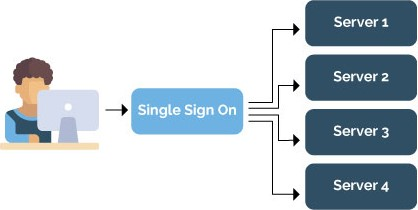
\includegraphics[width=0.7\linewidth]{img/SSOoverview.jpg}
\source{1}
\end{figure}

\end{itemize}
\end{frame}

\begin{frame}
\frametitle{Beispiel SSO Use Case}
\begin{itemize}
\item Eine Gruppe von Webseiten nimmt am SSO teil
\item Benutzer loggt sich auf einer dieser Website mit Passwort ein
\item Danach wird Benutzer auf anderen Websiten automatisch eingeloggt
\begin{figure}
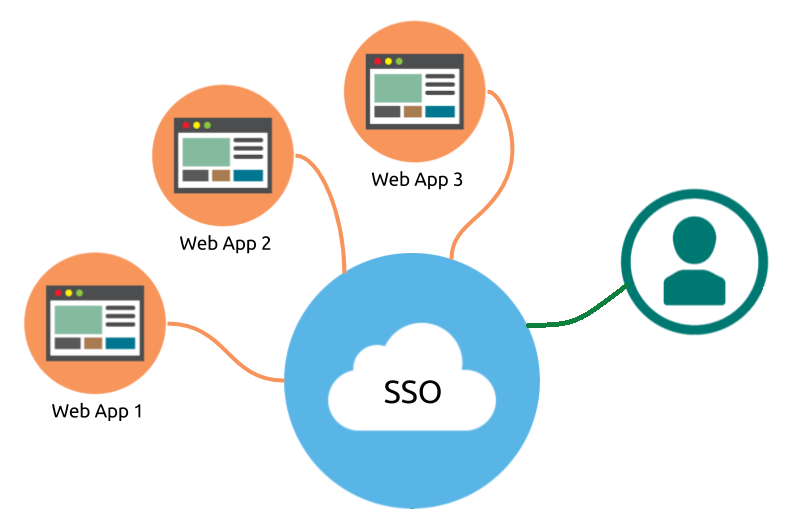
\includegraphics[width=0.7\linewidth]{img/SSOdiagram.png}
\source{2}
\end{figure}
\end{itemize}
\end{frame}
% jede dieser Webseiten stellt Dienste zur Verfügung, die für die authentifizierten und autorisierten Benutzer beschränkt ist
% müssen auch nicht nur Web Apps sein, das können auch Ressourcenserver sein, die auf einem entfernten Server laufen und die über eine REST API z.B. Ressourcen bereitstellen

\begin{frame}
\frametitle{Vorteile}
\begin{itemize}
\item Psychological Acceptability
\begin{itemize}
	\item Keine mehrfachen Anmeldungen
	\item Ein Passwort für mehrere Webanwendungen
\end{itemize}
\item Einfachere Entwicklung
\begin{itemize}
	\item Ein System zur Authentifizierung
\end{itemize}
\item Einfachere Administration
\begin{itemize}
	\item Alle Benutzerdaten an einem Ort
\end{itemize}
\end{itemize}
\end{frame}
% Psychological Acceptability: Sicherheitsmechanismen sollten allenfalls minimale Behinderungen einführen. Ansonsten ignorieren Endbenutzer diese Sicherheitsmechanismen
% Verschiedene passwörter merken führt zur Wahl einfacher Passwöter, hier hilft SSO bei dem man einen Benutzernamen und ein Passwort für mehrere Webanwendungen hat.

\begin{frame}
\frametitle{Nachteile}
\begin{itemize}
\item Single Point of Failure
\begin{itemize}
	\item Redundanz duch mehrere Keycloak Instanzen % TODO: Keycloak wurde hier noch nicht erklärt
\end{itemize}
\item Bereits existierende Systeme an SSO anbinden kann schwierig sein
\begin{itemize}
	\item Keycloak Adapter vereinfachen Anbindung
\end{itemize}
\end{itemize}
\end{frame}
% Keycloak bietet fertige Adapter für verschiedene Systeme und Programmiersprachen an. Diese Adapter vereinfachen die Anbindung von Systemen am SSO. % TODO: noch ein satz dazu sagen?

\begin{frame}
\frametitle{Alternativen}
\begin{itemize}
\item Verschiedene Arten von SSO
	\begin{itemize}
	\item SSO für Webanwendungen
	\item Alternative: SSO für Intranet/Enterprise
	\end{itemize}
\item Verschiedene Protokolle für SSO
	\begin{itemize}
	\item OpenID Connect (OIDC)
	\item Alternativen: SAML 2.0, Kerberos
	\end{itemize}
\item Verschiedene Implementierungen von SSO-Systemen
	\begin{itemize}
	\item Keine zwei SSO Implementierungen sind gleich
	\item Keycloak
	\item Alternativen: Okta, Auth0, Apereo CAS
	\end{itemize}
\end{itemize}
\end{frame}
% Nicht vollständig
% Es gibt verschiedene Möglichkeiten SSO umzusetzen.
% Diese Präsentation konzentriert sich auf SSO für Webanwendungen. Es gibt noch SSO für Intranet, was auch Enterprise SSO genannt wird. Dabei handelt es sich oft um native Anwendungen, die direkt auf dem Gerät des Benutzers laufen.
% OIDC und SAML 2.0 oder Kerberos
% Keycloak. Keycloak unterstützt sowohl das OIDC als auch das SAML 2.0 Protokoll. In der Beispielanwendung wird Keycloak ausschließlich mit OIDC verwendet
% Zusätzlich zu den SSO Features implementiert Keycloak auch Role Based Access Control. 
% Die Wahl der Implementierung für das SSO System ist wichtiger als man zunächst denkt, auch wenn die zur Auswahl stehenden Implementierung alle dasselbe Protokoll wie z.B. OIDC unterstützen. Denn es ist gerade >nicht< so, dass jede Implementierung die das OIDC Protokoll unterstützt genau gleich funktioniert. Der Grund dafür ist, dass das OIDC Protokoll manche Features als optional markiert. Die SSO Implementierung kann dann entscheiden welche optionalen Features implementiert werden. Zusätzlich werden manche Entscheidungen, z.B. wie sich der Benutzer authentifizieren soll, also z.B. über Username und Passwort, mit Zwei Faktor Authentifizierung, und so weiter, der SSO Implementierung überlassen. Da kann es  dann zwischen SSO Implementierung Unterschiede geben.
% Es ist auch so, dass die Implementierungen teilweise verschiedene oder teilweise nicht alle Sicherheitsfeatures enthalten. Das ist nicht immer schlecht, weil manchmal werden manche Sicherheitsfeatures aufgrund des Use Cases nicht benötigt. Aber da muss man dann halt schauen, welche Implementierung für seinen SSO Use Case infrage kommt, und bei unserem SSO für Webanwendungen ist Keycloak eine gute Wahl, wie wir dann auch später sehen werden.

\section{Aufbau von OpenID Connect}

\begin{frame}
\frametitle{OIDC Teilnehmer/Rollen}
\begin{itemize}
\item Benutzer
\item Clients
\item OpenID Provider
\end{itemize}
\end{frame}

\begin{frame}
\frametitle{Benutzer}
\begin{itemize}
\item Menschliche Teilnehmer
\item Kann sich einloggen
\item Benutzer hat Claims zugeordnet
\end{itemize}
\vspace{15pt}
\begin{figure}

\includegraphics[width=0.2\linewidth]{img/usericon.png}
\source{3}
\end{figure}
\end{frame}
% usericon.webp
% menchschliche teilnehmer bei der Authentifizierung

\begin{frame}
\frametitle{Claims}
\begin{itemize}
\item Key-Value Paare
\item Information über Benutzer, z.B. Name, Adresse, email
\item Information über Authentifizierung, z.B. wann und bei wem hat Authentifizierung des Benutzers stattgefunden
\item Beispiel Claims:
	\begin{itemize}
	\item 'sub' (Subject) Claim: Benutzer ID, erstellt von Issuer
	\item 'iss' (Issuer) Claim: Bei welcher Instanz authentifiziert
	\end{itemize}
\end{itemize}
\begin{figure}
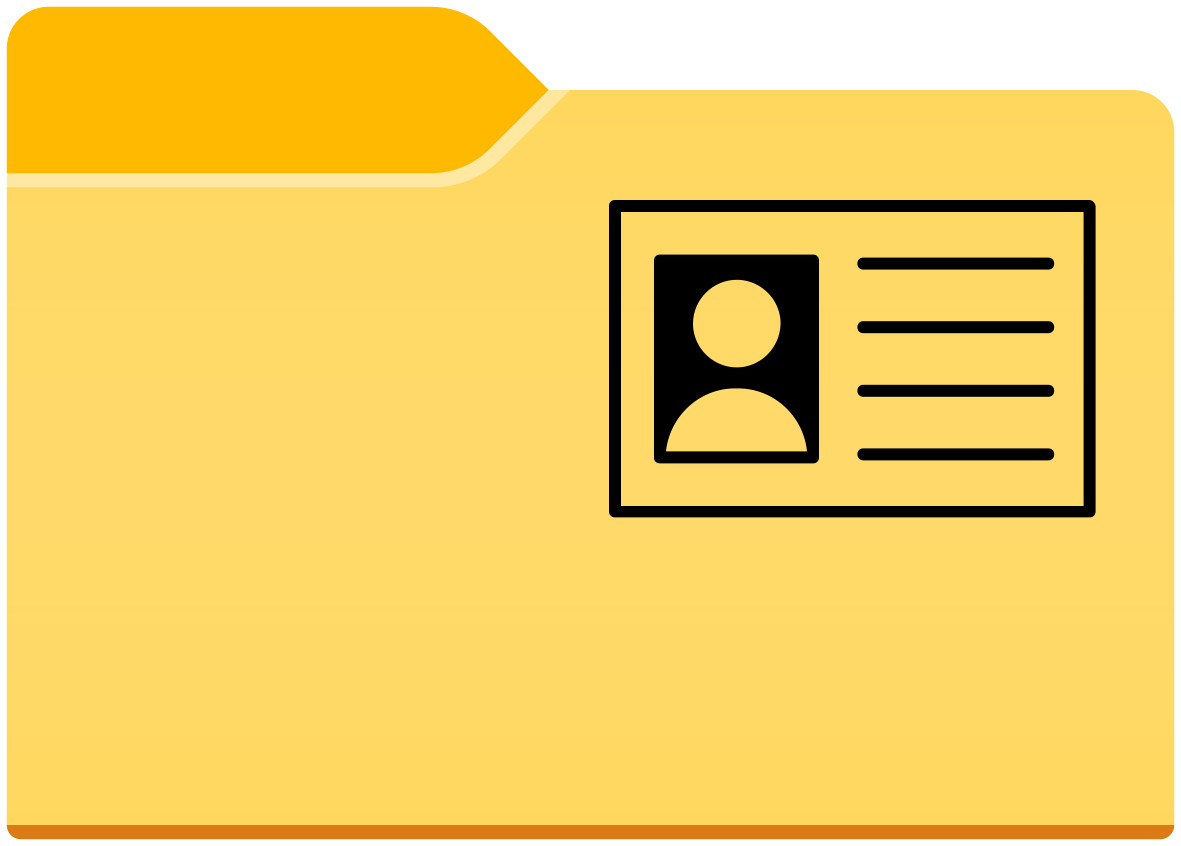
\includegraphics[width=.3\linewidth]{img/userdatafolder.png}
\source{7}
\end{figure}
\end{frame}
% 'iss' (Issuer) Claim: ID der Instanz, bei der sich der Benutzer authentifiziert hat

\begin{frame}
\frametitle{Clients}
Drei Arten von Clients:
\begin{enumerate}
\item Ruft andere Clients/Services im Namen des authentifizierten Benutzers auf
	\begin{itemize}
	\item z.B. Frontend Anwendungen
	\item Rufen geschützte Ressourcen von Backend Services ab
	\end{itemize}
\item Backend Services die Ressourcen bereitstellen
	\begin{itemize}
	\item z.B. Ressourcenserver
	\item Ressourcen beschränkt für authentifizierte und authorisierte Benutzer
	\end{itemize}
\item Native Anwendungen
	\begin{itemize}
	\item Laufen auf Gerät des Benutzers
	\item Für Web SSO nicht interessant
	\end{itemize}
\end{enumerate}

\begin{figure}
\centering
\begin{minipage}{.3\textwidth}
\centering
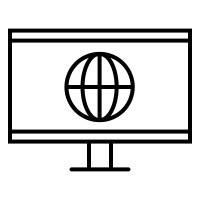
\includegraphics[width=.5\linewidth]{img/clienticon.png}
\end{minipage}%
\begin{minipage}{.3\textwidth}
\centering

\includegraphics[width=.5\linewidth]{img/web-service-icon-9.jpg}
\end{minipage}
\source{4, 5}
\end{figure}

\end{frame}



\begin{frame}
\frametitle{OpenID Provider}
\begin{itemize}
\item Authentifiziert Benutzer
\item Speichert z.B. Claims der Benutzer und Konfiguration der Clients
\item Stellt Endpunkte bereit für:
	\begin{itemize}
	\item Authentifizierung eines Benutzers
	\item UserInfo Endpunkt (Informationen über Benutzer)
	\item Token Endpunkt (Tokens mit späterer Verfallszeit und/oder weniger Rechten)
	\end{itemize}
\end{itemize}
\vspace{15pt}
\begin{figure}

\includegraphics[width=.5\linewidth]{img/keycloaklogo.png}
\source{6}
\end{figure}
\end{frame}

\begin{frame}
\frametitle{Tokens}
\begin{itemize}
\item Tokens im JWT-Format
\item Erstellt und Signiert vom OpenID Provider
\item Verschiedene Arten von Tokens:
	\begin{itemize}
	\item ID Token
	\item Access Token
	\item Refresh Token
	\end{itemize}
\item 3 teilige Struktur:
\begin{figure}
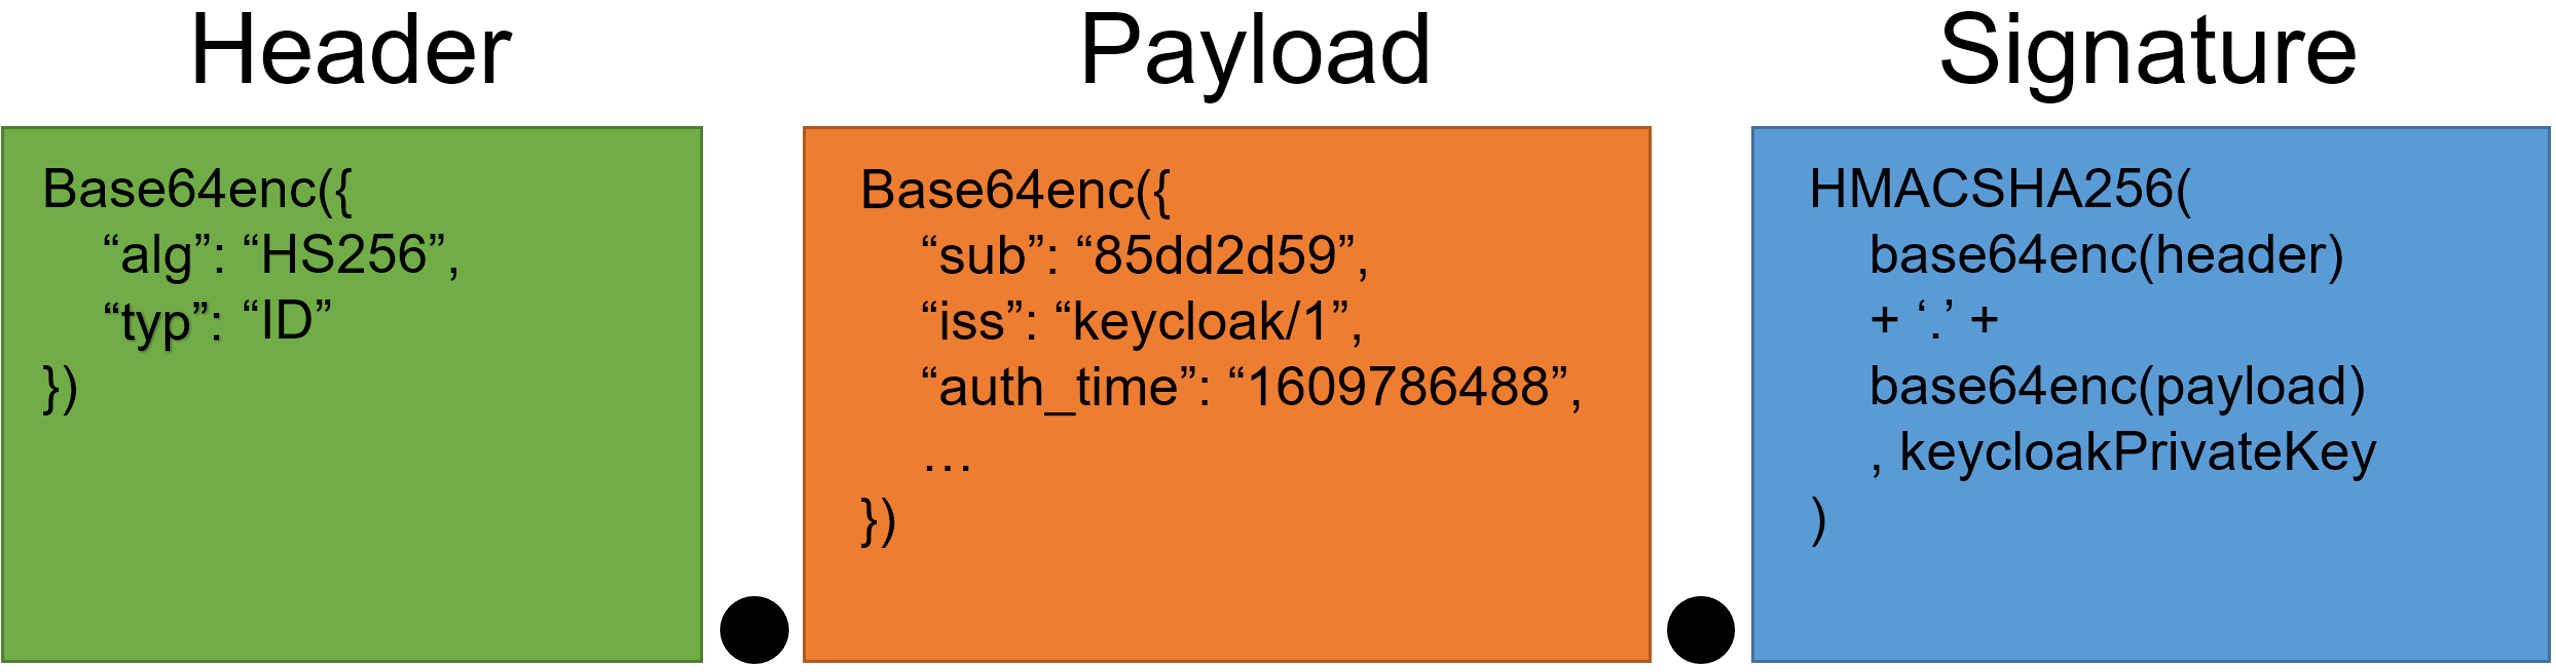
\includegraphics[width=1\linewidth]{img/jwttoken.png}
\source{8}
\end{figure}
\end{itemize}
\end{frame}
% Header - enthält z.B. verwendeter Signaturalgorithmus
% Payload: Menge von JWT Claims
% Signatur von Teil 1 und 2

\begin{frame}
\frametitle{ID Token}
\begin{itemize}
\item Enthält Claims über die Authentifizierung des Benutzers
	\begin{itemize}
	\item z.B. 'auth\_time' Claim: Wann hat Authentifizierung stattgefunden
	\end{itemize}
\item Optional weitere Claims mit Informationen über den Benutzer
\item Ist nur für den an der Authentifizierung des Benutzers beteiligten Client gedacht
\item Client validiert mit ID Token die Authentifizierung des Benutzers
\end{itemize}
\begin{figure}

\includegraphics[width=.3\linewidth]{img/idtoken.png}
\source{9}
\end{figure}
\end{frame}

\begin{frame}
\frametitle{Access Token}
\begin{itemize}
\item Schlüssel für Ressourcen, welche für die authentifizierten und authorisierten Benutzer beschränkt ist
\item Kann z.B. als Bearer Token im HTTP Authorization Header an Backend Services enthalten sein
\item Sollte außer 'sub' Claim keine Informationen über Benutzer enthalten
\item Informationen über Benutzer kann mit Access Token bei UserInfo Endpunkt angefordert werden
\item Enthält 'scope' Claim
	\begin{itemize}
	\item Spezifiziert Ressourcen und Benutzer Claims
	\item Mit Access Token Zugriff hat man auf Spezifiziertes Zugriff
	\item Ressourcen bei Backend Services 
	\item Benutzer Claims bei UserInfo Endpunkt
	\end{itemize}
\end{itemize}
\end{frame}

\begin{frame}
\frametitle{Access Token}
\begin{figure}
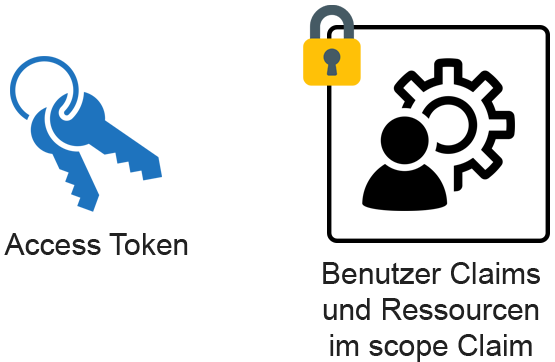
\includegraphics[width=.7\linewidth]{img/accesstokeniconfull.png}
\source{10, 11}
\end{figure}
\end{frame}
% Wie gesagt, nicht jeder Schlüssel passt zu jedem Schloss => access token nur für bestimmte (scope claim) ressourcen und benutzer claims

\begin{frame}
\frametitle{Refresh Token}
\begin{itemize}
\item OIDC Tokens haben Verfallszeit ('exp' Claim)
\item Abgelaufene Tokens sind nicht mehr gültig
\item Mit Refresh Tokens können über den Token Endpunkt neue Tokens angefordert werden
	\begin{itemize}
	\item Optional neue Tokens mit weniger Rechten
	\end{itemize}
\end{itemize}
\vspace{25pt}
\begin{figure}

\includegraphics[width=.2\linewidth]{img/Refreshicon.png}
\source{12}
\end{figure}
\end{frame}
% Optional neue Tokens mit weniger Rechten für z.B. Access Token an weniger vertrauenswürdigen client

\begin{frame}
\frametitle{OIDC Protokoll Flows}
\begin{itemize}
\item Authorization Code Flow
\item Zugriff auf geschützte Ressourcen
\item Validieren des Access Tokens
\end{itemize}
\end{frame}

\makeatletter
\newcommand*{\centerfloat}{%
  \parindent \z@
  \leftskip \z@ \@plus 1fil \@minus \textwidth
  \rightskip\leftskip
  \parfillskip \z@skip}
\makeatother

\begin{frame}
\frametitle{Authorization Code Flow Schritt 1}
\begin{figure}
\centerfloat
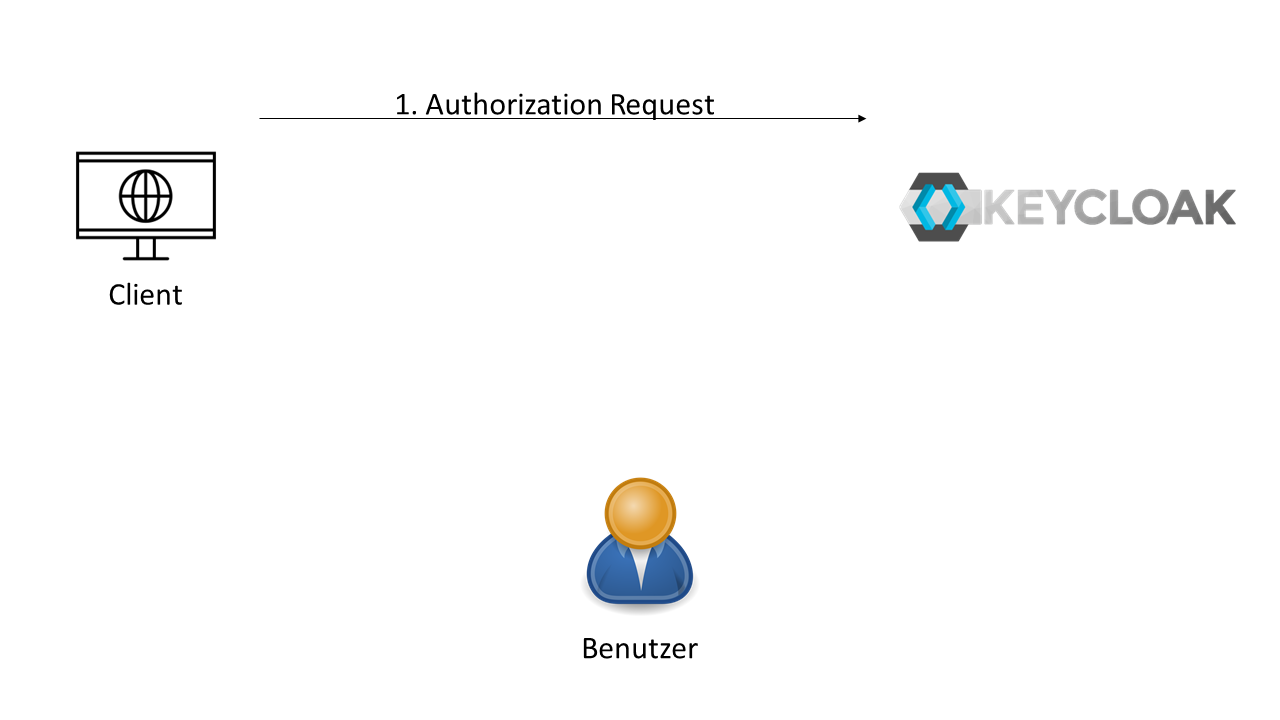
\includegraphics[width=1.1\linewidth]{img/authflow1.png}
\end{figure}
\end{frame}

\begin{frame}[fragile]
\frametitle{Authorization Code Flow Schritt 1 Beispiel}
\begin{lstlisting}[caption=Beispiel Authorization Request, captionpos=b, label=EBAuthorizationRequest]
GET https://keycloak/auth/realms/.../auth?
        client_id=frontend1
        &redirect_uri=https%3A%2F%2Ffrontend.com%2F
        &state=0909ff6a-53b2-4253-8690-aff72d2cfff1
        &response_mode=fragment
        &response_type=code
        &scope=openid%20profile
        &nonce=67bad316-d8c1-45d1-9559-2a1c4726ce91
\end{lstlisting}
\end{frame}
% GET Anfrage, das bedeutet, der Benutzer ist nach dem Authorization Request auf der Seite von Keycloak.

\begin{frame}
\frametitle{Authorization Code Flow Schritt 2}
\begin{figure}
\centerfloat
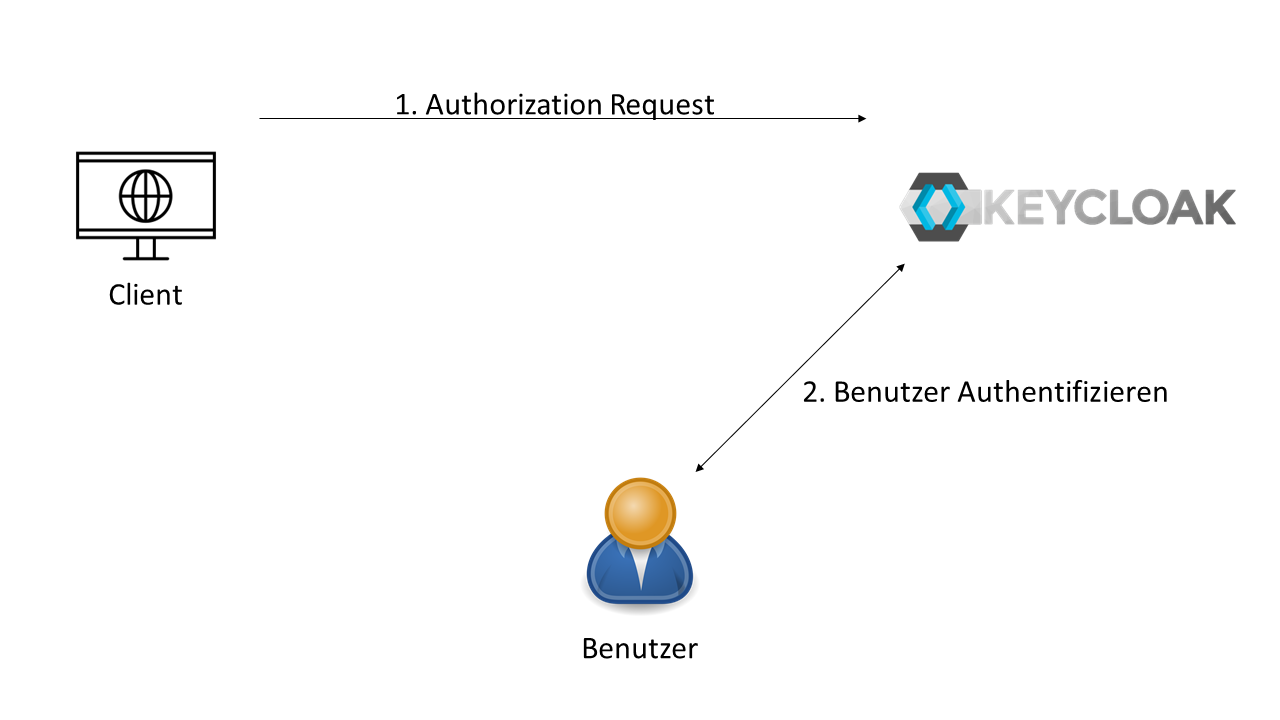
\includegraphics[width=1.1\linewidth]{img/authflow2.png}
\end{figure}
\end{frame}
% Das ist wichtig, denn im nächsten Schritt, bei der authentifizierung des Benutzers, gibt der Benutzer z.B. sein Passwort ein. Da das nicht auf der Seite des Clients passiert, sind die Anmeldeinformationen des Benutzers vom Client abgeschirmt. Der Client arbeitet nur mit Tokens und nicht mit Anmeldeinformationen wie Benutzername und Passwort.

\begin{frame}
\frametitle{Authorization Code Flow Schritt 3}
\begin{figure}
\centerfloat
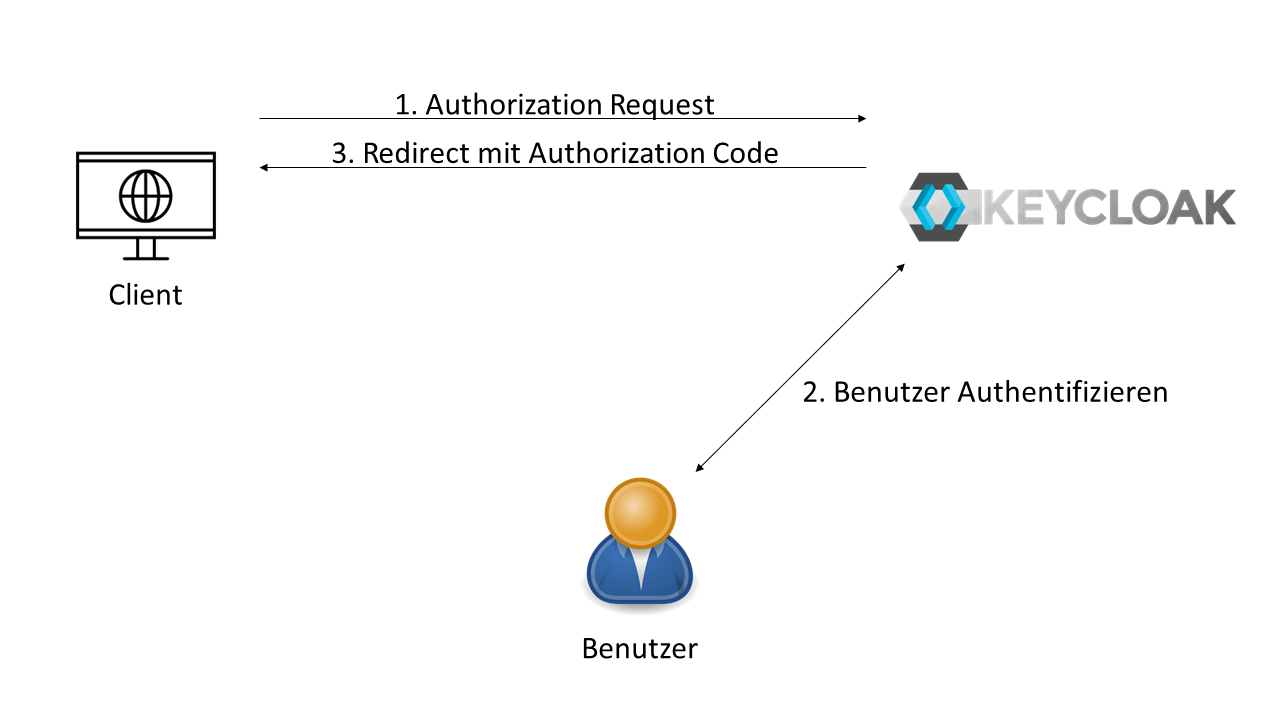
\includegraphics[width=1.1\linewidth]{img/authflow3.png}
\end{figure}
\end{frame}

\begin{frame}
\frametitle{Authorization Code Flow Schritt 4}
\begin{figure}
\centerfloat
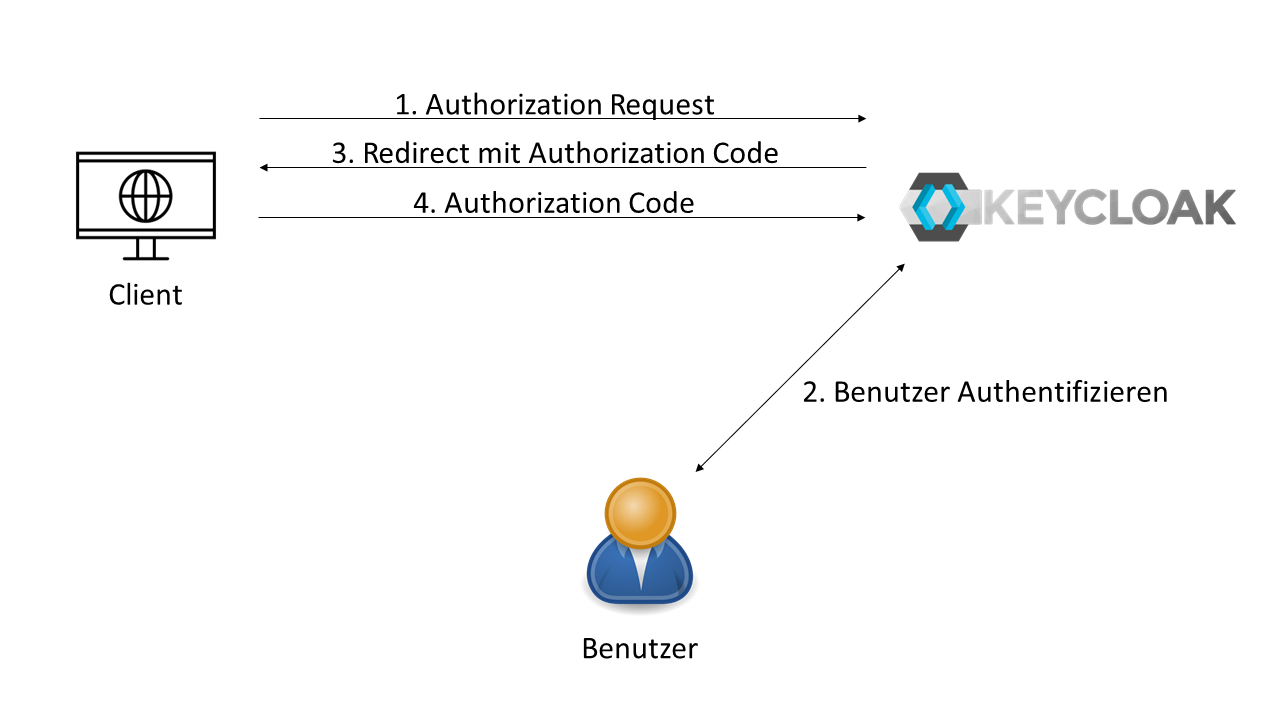
\includegraphics[width=1.1\linewidth]{img/authflow4.png}
\end{figure}
\end{frame}
% Durch die POST Anfrage werden die Tokens im HTTP Response Body zurückgegeben. Dadurch werden sie nicht dem Browser ausgesetzt. Um potenzielle Replay Angriffe zu verhindern, kann dieser Authorization Code nur einmal verwendet werden und hat eine sehr kurze Verfallszeit

\begin{frame}
\frametitle{Authorization Code Flow Schritt 5}
\begin{figure}
\centerfloat
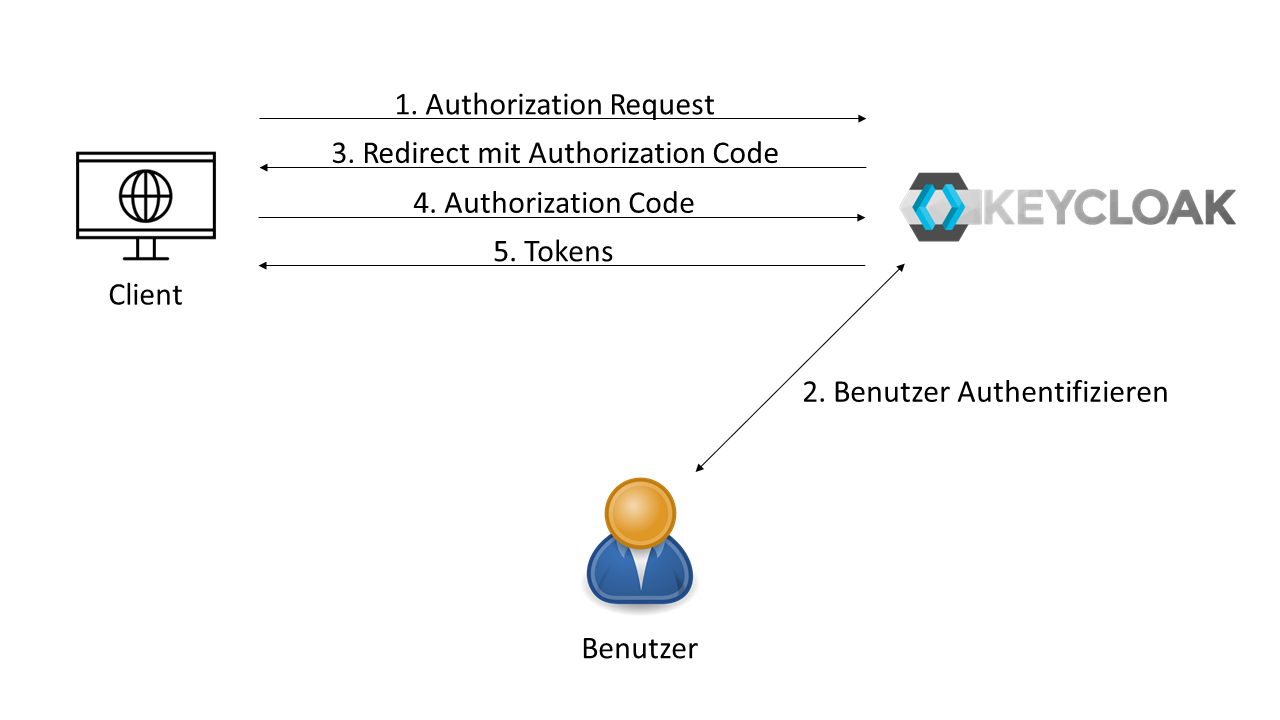
\includegraphics[width=1.1\linewidth]{img/authflow5.png}
\end{figure}
\end{frame}
% Danach noch ID Token validieren

\begin{frame}
\frametitle{Zweite Authentifizierung}
\begin{itemize}
\item Nach erster erfolgreicher Authentifizierung wird Cookie mit ID Token für Keycloak's Authorization Endpunkt gesetzt
\end{itemize}
\begin{figure}
\centerfloat
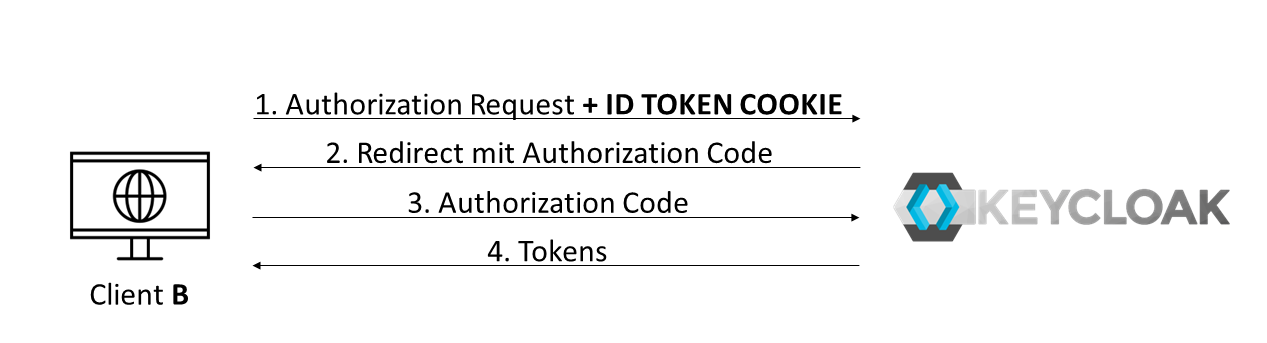
\includegraphics[width=1.1\linewidth]{img/authflow6.png}
\end{figure}
\end{frame}

\begin{frame}
\frametitle{Zugriff auf geschützte Ressourcen}
\begin{itemize}
\item Access Token im Authorization Header der HTTP Anfrage
\item Jeder kann Access Token einsetzen
% TODO: img von microservice architektur
\item Einschränken der abrufbaren Ressourcen und Benutzer Claims durch 'scope' und Audience Claims des Access Tokens
\item Empfänger muss 'scope' und Audience Claims überprüfen
\end{itemize}
\end{frame}
% Empfänger der HTTP Anfrage mit dem Access Token muss 'scope' und Audience Claims überprüfen, und das, bevor er die Ressourcen und Benutzer Claims zurücksendet.

\begin{frame}
\frametitle{Validieren des Access Tokens - Offline Variante}
\begin{figure}
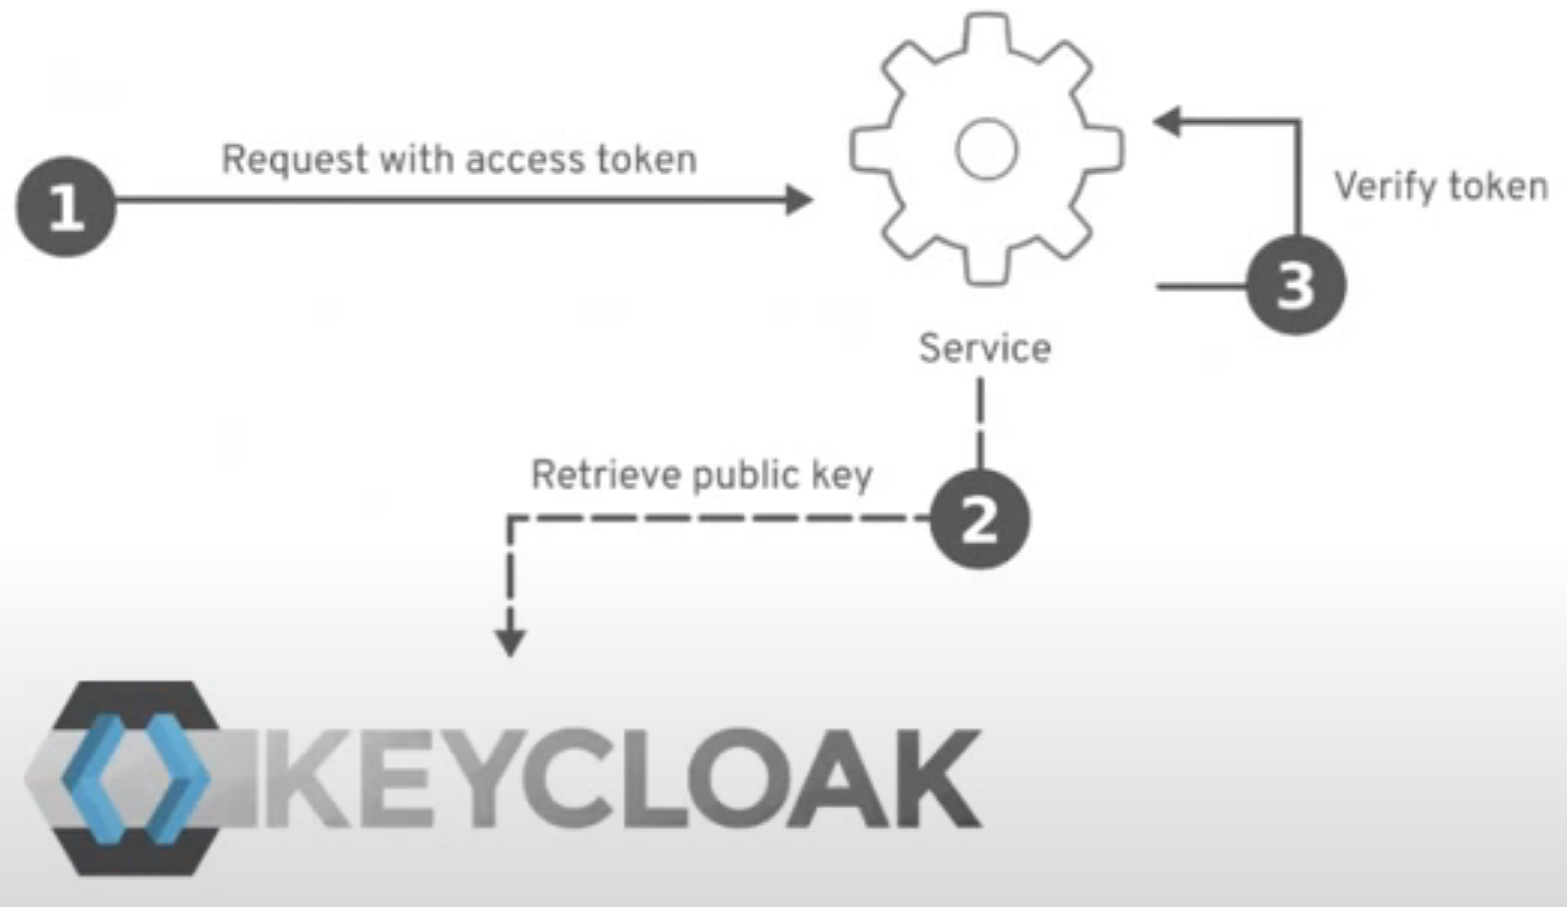
\includegraphics[width=.7\linewidth]{img/VerifyAccessTokenOffline.PNG}
\source{13}
\end{figure}
\begin{itemize}
\item Public Key gecached
\item Verringerte Latenz
\item Verringerte Auslastung des Keycloak Servers
\item Access Token kann nicht wiederrufen und invalidiert werden
\end{itemize}
\end{frame}
% Aus diesem Grund haben Access Tokens im OpenID Connect Protokoll eine kurze Verfallszeit

\begin{frame}
\frametitle{Validieren des Access Tokens - Online Variante}
\begin{figure}
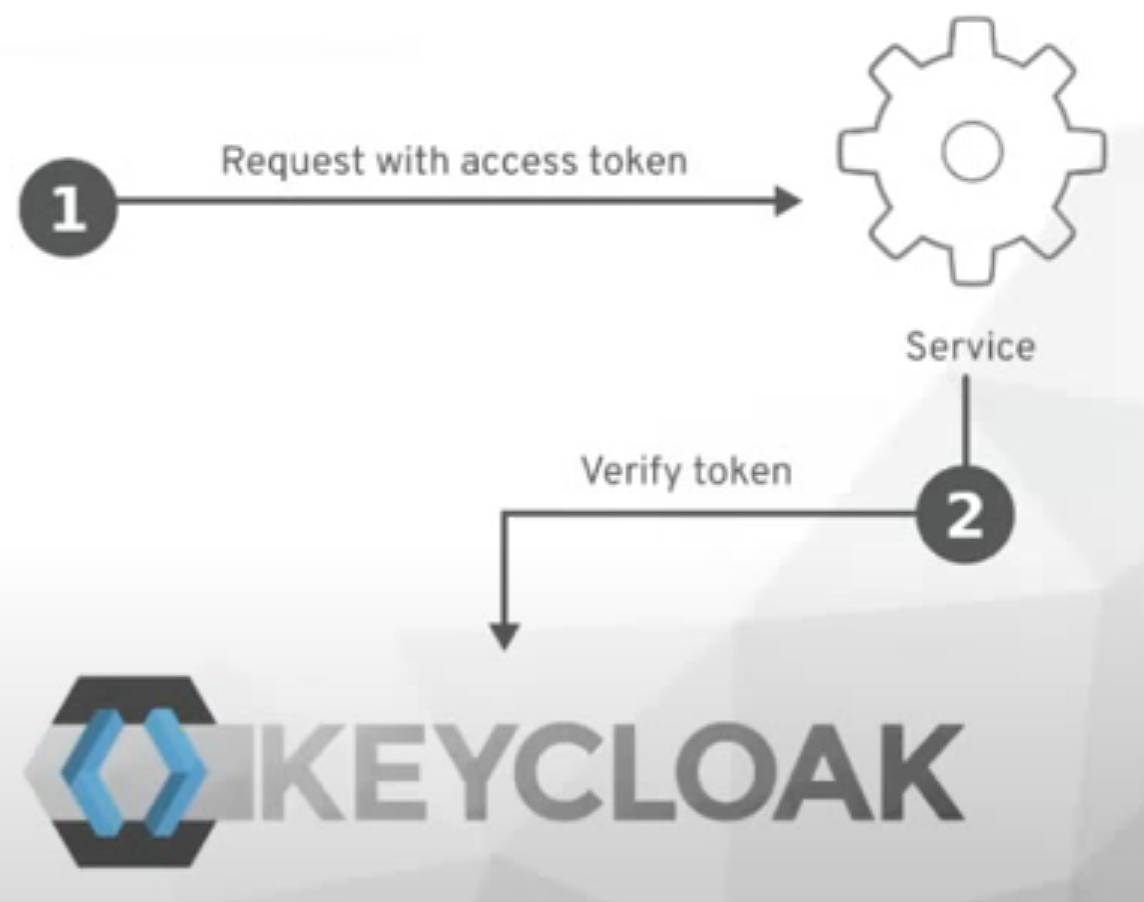
\includegraphics[width=.5\linewidth]{img/VerifyAccessTokenOnline.PNG}
\source{13}
\end{figure}
\begin{itemize}
\item Höhere Latenz
\item Höhere Auslastung des Keycloak Servers
\item Access Token kann wiederrufen und invalidiert werden
\end{itemize}
\end{frame}

\section{Threat Model}

\begin{frame}
\frametitle{Threat Model}
\begin{itemize}
\item Client Schwachstellen
\item Authorization Server Schwachstellen
\item Token Schwachstellen
\end{itemize}
\end{frame}

% OIDC keine Kryptographie drin hat > TLS/HTTPS verschlüsseln muss
% Diebstahl von Tokens
% Folge von Diebstahl der Bearer Tokens

% XSS: Tokens an Angreifer schicken, zwar keine Logindaten, aber tokens dann kann sich Angreifer als anderer Benutzer ausgeben
% CSRF: state param thing?

%OIDC und OAuth 2.0 sind frei von Kryptographie. Stattdessen verlassen sich die Protokolle vollständig auf das Vorhandensein von TLS über die verschiedenen Verbindungen hinweg. Aus diesem
%Grund gilt es die Verwendung von TLS im gesamten System so weit wie möglich durchzusetzen. Dabei kann HTTP Strict Transport Security (HSTS) helfen. HSTS erlaubt es zu definieren, dass Browser oder andere konforme User-Agents nur über sichere HTTPS-Verbindungen interagieren sollten und niemals über das unsichere HTTP-Protokoll. HSTS kann über den zusätzlichen HTTPHeader Strict-Transport-Security hinzugefügt werden. Jedes Mal, wenn versucht wird, den Endpunkt des Client-Backends mit dem Browser über HTTP zu erreichen, würde der Browser einen Redirect zu HTTPS durchführen. Dadurch wird jede unerwartete unverschlüsselte Kommunikation (wie z.B. Protokoll-Downgrade-Angriffe) vermieden.

\begin{frame}
\frametitle{Client Schwachstellen}
\begin{itemize}
\item Cross-Site-Request-Forgery (CSRF)
	\begin{itemize}
	\item Z.B. Angreifer sendet gefälschte Authentifizierungsantwort an Client's redirect URI
	\item State Token (Anti-CSRF Token)
	\end{itemize}
\item Registrierung der redirect\_uri
	\begin{itemize}
	\item Angreifer gibt sich als Client aus
	\item Möglich wenn redirect\_uri zu unspezifisch
	\end{itemize}
\item Diebstahl von Tokens 
	\begin{itemize}
	\item Z.B. durch XSS
	\end{itemize}
\item OIDC frei von Kryptographie
	\begin{itemize}
	\item Verwendung von TLS voraussetzen, z.B. mit HSTS
	\end{itemize}
\end{itemize}
\end{frame}
% A CSRF attack against the client's redirection URI allows an attacker to inject its own authorization code or access token, which can result in the client using an access token associated with the attacker's protected resources rather than the victim's (e.g., save the victim's bank account information to a protected resource controlled by the attacker). That value allows you to prevent the attack by confirming that the value coming from the response matches the one you sent.
% It prevents an attack where the attacker produces a fake authentication response, e.g. as part of the Basic Client Profile by sending a code to the Client's redirect URI. For example: after phishing the user an attacker could inject a stolen code that would be associated with the current user in this way. The state correlates request and response so an unsolicited crafted response is not possible without knowing the state parameter that was used in the request.
% State Token, auch Anti CSRF Token genannt. CSRF macht ja eine andere gruppe darum will ich da nicht ins detail gehen

\begin{frame}
\frametitle{Authorization Server Schwachstellen}
\begin{itemize}
\item Redirection URI manipulieren
	\begin{itemize}
	\item Authorization Code zu URI des Angreifers umleiten
	\end{itemize}
\item Session Hijacking
	\begin{itemize}
	\item Z.B. Authorization Code aus Browser-Verlauf auslesen
	\item Deshalb darf Authorization Code nur einmal eingelöst werden %für tokens und ist danach ungültig
	\end{itemize}
\end{itemize}
\end{frame}

\begin{frame}
\frametitle{Token Schwachstellen}
\begin{itemize}
\item Token Modification
	\begin{itemize}
	\item Empfänger von Access Token muss digitale Signatur überprüfen
	\end{itemize}
\item Token Replay
	\begin{itemize}
	\item Gute Verschlüsselung, geringe Token Verfallszeit
	\end{itemize}
\item Token Redirect
	\begin{itemize}
	\item Empfänger ID im Token % TODO: was ist das?
	\end{itemize}
\item Token Disclosure
	\begin{itemize}
	\item Token selbst könnte sensible Informationen enthalten
	\end{itemize}
\end{itemize}
\end{frame}
% Token Replay: Sobald eine Anfrage mit Access Key geknackt ist, kann Access Key vom Angreifer wiederverwendet werden (vorrausgesetzt nicht Token abgelaufen). Nicht nur Inhalt der nachricht, z.B. Ressource wird offengelegt, sondern token kann auch weiterverwendet werden für Ressourcen die vom Client nie angefordert wurden.

\section{Demo von SSO innerhalb einer Beispielwebanwendung}

\begin{frame}
\frametitle{Notiz an Herr Professor Karg}
\begin{itemize}
\item Notiz an Herr Professor Karg: Abschließend folgt noch eine Demo der implementierten Beispielwebanwendung in der VM. Vom Inhalt wird diese Demo ungefähr so sein wie das Kapitel 1.4 "Umsetzung von SSO innerhalb einer Beispielwebanwendung" unserer Ausarbeitung.
\end{itemize}
\end{frame}

% TODO: eventuell zusammenfassung slide

\begin{frame}
\frametitle{Quellen Teil 1}
\begin{itemize}
\item [1] https://www.renovodata.com/blog/2019/01/17/single-sign-on
\item [2] https://insready.com/en/blog/single-sign-using-oauth2-and-jwt-distributed-architecture
\item [3] https://commons.wikimedia.org/wiki/File:User\_icon\_2.svg
\item [4] https://thenounproject.com/term/web-application/3085910/
\item [5] https://icon-library.com/icon/web-service-icon-9.html
\item [6] https://design.jboss.org/keycloak/logo/images/ keycloak\_logo\_600px.png
\end{itemize}
\end{frame}

\begin{frame}
\frametitle{Quellen Teil 2}
\begin{itemize}
\item [7] https://upload.wikimedia.org/wikipedia/commons/5/59/ OneDrive\_Folder\_Icon.svg; user data icon by Mohamad Arif Prasetyo from the Noun Project
\item [8] https://www.toptal.com/web/cookie-free-authentication-with-json-web-tokens-an-example-in-laravel-and-angularjs
\item [9] https://iconarchive.com/show/job-seeker-icons-by-inipagi/id-card-icon.html
\item [10] https://de.cleanpng.com/png-jry6v5/
\item [11] https://thenounproject.com/search/?q=resource\&i=2979093 resource by Hrbon from the Noun Project
\item [12] https://commons.wikimedia.org/wiki/File:Refresh\_icon.svg
\item [13] https://www.youtube.com/watch?v=mdZauKsMDiI
\end{itemize}
\end{frame}

\begin{comment}
\begin{frame}
\frametitle{TITLE}
\begin{itemize}
\item ITEM
\end{itemize}
\end{frame}
\end{comment}


%------------------------------------------------

\begin{frame}
\Huge{\centerline{Danke \& Ihre Fragen}}
\end{frame}

%----------------------------------------------------------------------------------------

\end{document}

%%% Local Variables: 
%%% mode: latex
%%% TeX-PDF-mode: t
%%% TeX-master: t
%%% TeX-engine: xetex
%%% End: 
